\documentclass[10pt,twocolumn,letterpaper]{article}

\usepackage{cvpr}
\usepackage{times}
\usepackage{epsfig}
\usepackage{graphicx}
\usepackage{amsmath}
\usepackage{amssymb}

% Include other packages here, before hyperref.

% If you comment hyperref and then uncomment it, you should delete
% egpaper.aux before re-running latex.  (Or just hit 'q' on the first latex
% run, let it finish, and you should be clear).
\usepackage[breaklinks=true,bookmarks=false]{hyperref}

\cvprfinalcopy % *** Uncomment this line for the final submission

\def\cvprPaperID{****} % *** Enter the CVPR Paper ID here
\def\httilde{\mbox{\tt\raisebox{-.5ex}{\symbol{126}}}}

% Pages are numbered in submission mode, and unnumbered in camera-ready
%\ifcvprfinal\pagestyle{empty}\fi
\setcounter{page}{1}
\begin{document}
	
%%%%%%%%% TITLE\
\title{Term Project Report \\
Normal Map Estimation using Model Geometry and Texture \\
Team: Avengers }
\author{Jang Wonjong, Lee Dahun, Jacob Morton\\
	20140337, 20130221, 20172327\\
	Computer Science and Engineering, POSTECH\\
	{\tt\small}}

\maketitle
%\thispagestyle{empty}

%%%%%%%%% BODY TEXT
\section{Introduction}
\begin{figure}[t]
	\begin{center}
		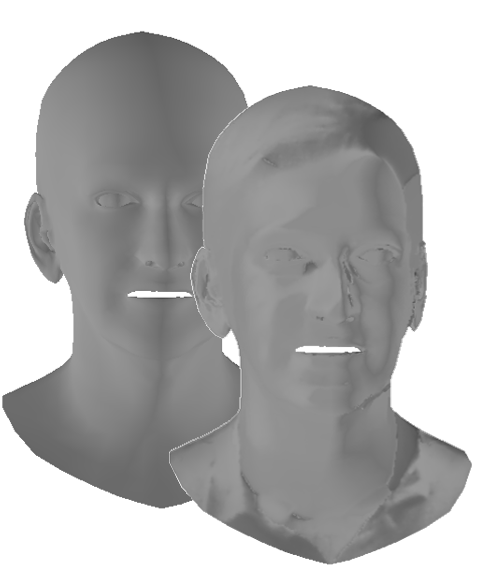
\includegraphics [scale=0.5] {image/intro.png}
	\end{center}
	\caption{Example of a face model with \textbf{Left:} Geometry only, \textbf{Right:} Geometry + Normal Map}
	\label{fig:title}
\end{figure} 

\subsection{Motivation}
 There are several tools available to generate 3D models and textures, like 3D Studio Max, Maya, blender, and Adobe Photoshop. It is not too difficult to program or load these into OpenGL as well. The problem of using 3D geometry and Texture alone is that it can produce flat looking renderings, especially if the geometry is less detailed than the texture. This is typically the case, as texturing can hide simple or flawed geometry. There is more we can do with texture mapping than just wrapping the geometry with an RGB image. We can also add bump maps, normal maps, displacement maps, and even subsurface scattering to make the rendering more realistic. But these additional mappings are difficult to produce and are often hand-made or produced in multi-step procedures, i.e. baking. Using detailed normal maps in addition to texture can improve the perceptual quality of 3D reconstructed scenes and objects while being illuminated by a light source. We wish for there to be a simple automated procedure that can take an RGB picture with a geometric prior and produce a high-quality normal map. Such a tool would be useful in entertainment and 3D Reconstruction.


\subsection{Project Description}
Inspired by Shape-From-Shading, we propose a tool for estimating a normal map from a given texture. We extract interpolated normals from a geometric prior. We use off-the-shelf intrinsic image decomposition to estimate the albedo texture and remove shading from a single photograph. Given the albedo and interpolated normals, we use spherical harmonics to alternatively estimate the environment illumination first and then compute a per-pixel normal map second. We can then apply this normal map to the model in addition with texture during the texturing process. We demonstrate this by using a fragment shader in OpenGL. \par
This project requires knowledge in Intrinsic Image Decomposition, Spherical Harmonics (SH), least-squares optimization, and illumination and normal mapping in OpenGL using fragment shaders.

\section{Development Environment}
Our illumination estimation and normal refinement code is publicly available on the github repository \url{https://github.com/spacejake/cg-project}.
\begin{table}[h]
	\begin{tabular}{ll}
		\textbf{Operating System:} &  Windows 10  \\
		\textbf{IDE:} &  MS Visual Studios 2017  \\
        &PyCharm\\
		\textbf{Libraries:} &  OpenGL, FreeGlut, GLEW, GLM,\\
		&chumpy
	\end{tabular}
\end{table}

\section{Overview}
\subsection{Intrinsic Image Decomposition}
 We also need a good approximation of the albedo texture $\rho(x,y)$, but it is difficult to acquire as we need an image without shading. We will pre-process the RGB image to remove shading $s(x,y)$ using widely available open-source intrinsic image decomposition\cite{bell}. intrinsic image decomposition is used to decompose an image into reflectance (albedo) and shading images, and is typically formulated as 
\begin{equation}
I(u,v) = \rho(u,v)s(u,v),
\end{equation}
Where $I(u,v)$ is the input raw image with shading from a lit environment. 
\begin{figure}[!h]
    \begin{center}
        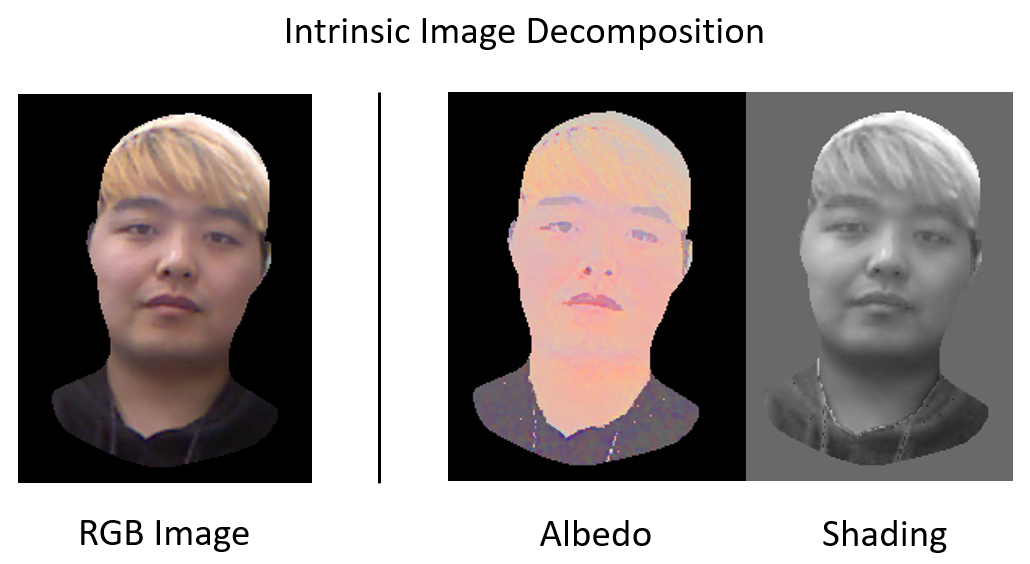
\includegraphics [scale=0.3] {image/intrinsic.png}
    \end{center}
    \caption{Decompose image $I$ into albedo $\rho$ and shading $s$}
    \label{fig:intrinsic}
\end{figure} 

\begin{figure*}[t]
    \begin{center}
        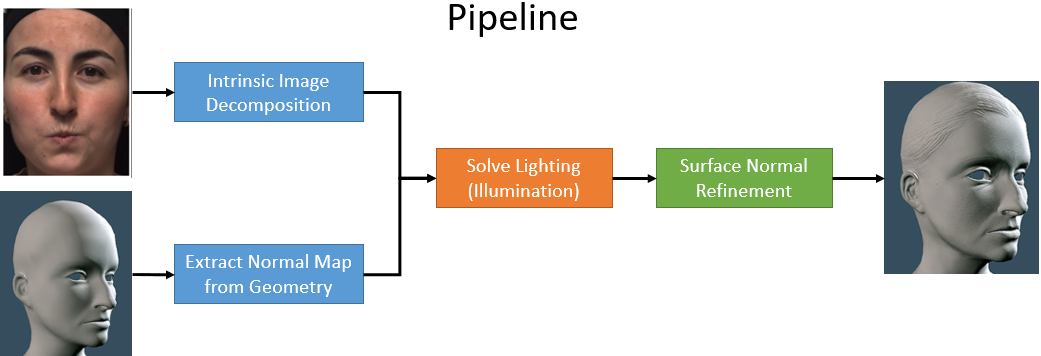
\includegraphics [scale=0.7] {image/pipeline.png}
    \end{center}
    \caption{Pipeline}
    \label{fig:pipe1}
\end{figure*} 
\subsection{Spherical Harmonics}
\begin{figure}[h]
    \begin{center}
        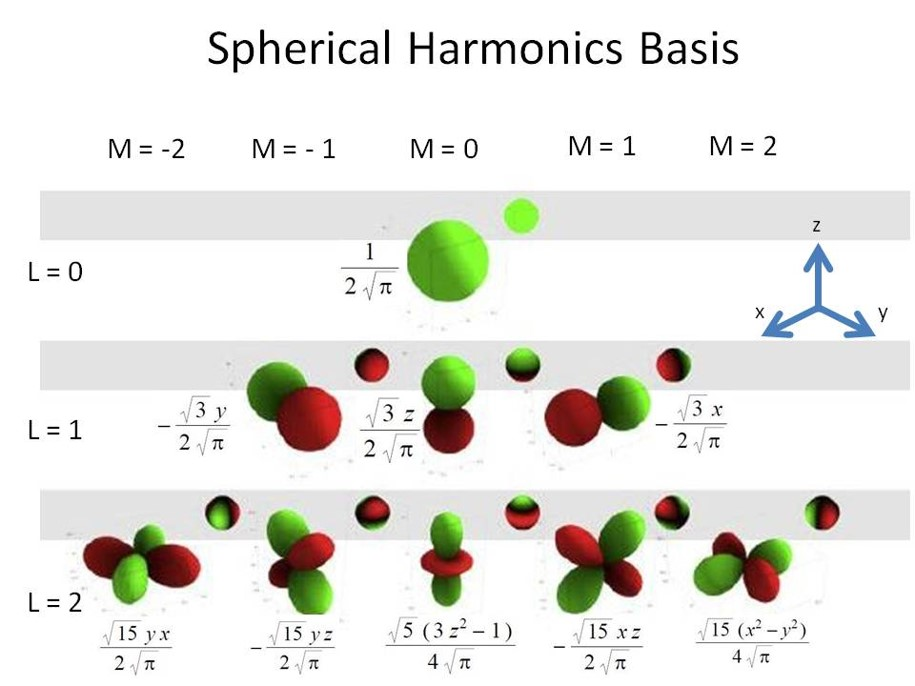
\includegraphics [scale=0.5] {image/sh_basis.jpg}
    \end{center}
    \caption{L the band (order), M is the degree (basis)}
    \label{fig:sh-basis}
\end{figure} 
Spherical harmonics are a set of harmonic functions defined on the surface of a sphere. Many surfaces are mostly diffuse, so we assume Lambertion diffuse surfaces. We will be using the Real and Cartesian form of $2^{nd}$-order spherical harmonics. The first band represents ambient energy, the remaining bands represent more and more complex diffuse reflectance. The Lambertian factor $a_l$ acts as a blur kernel reducing the energy at higher orders. \par
Spherical harmonics is a common method for illumination and geometric refinement. The spherical harmonics reflectance model is widely adopted in many areas of computer graphics, from rendering to 3D reconstruction. We can estimate diffuse illumination parameters of an image scene, given some rough geometric assumptions. Illumination is assumed to be multiple light sources at an infinite distance. We can also measure energy at each pixel on an image to determine the pixel's normal vector when illumination is roughly known. Spherical harmonics is commonly used in single image Shape-from-Shading methods due to these properties. The first 3 bands of spherical harmonics are most typically used, which represent reflectance sufficiently in most cases.
We will use the geometric prior to extract the initial normal map $N_{ref}$.  Given $N_{ref}$ and $\rho(x,y)$, we will solve the least-squares problem to estimate lighting parameters $L_l^m$,
\begin{equation}
I = \rho \sum_{l,m} a_l L_m^l Y_m^l(N_{ref}),
\end{equation}
where $Y(n_x,n_y,n_z)$ is the spherical harmonics basis function. After lighting has been estimated, we will solve for the normal map by refining $N_{ref}$ to produce $N$, the recovered lighting parameters $L_l^m$, and $\rho$,
\begin{equation}
I = \rho \sum_{l,m} a_l L_m^l Y_m^l(N).
\end{equation}
We will render the resulting normal map $N$ in OpenGL using a fragment shader. We represent a per-pixel formulation in uv-coordinates,
\begin{equation}
I(u,v) = \rho(u,v) \sum_{l,m} a_l L_m^l Y_m^l(n(u,v)).
\end{equation}
The set of real spherical harmonics basis functions in Cartesian space $Y_m^l$ for the first 3 bands are defined \cite{sfs} as 
\begin{equation}
\begin{split}
&Y_0^0 = c_0\\
&Y_1^{-1} = c_1 n_x\\
&Y_1^{0} = c_1 n_y\\
&Y_1^{1} = c_1 n_z\\
&Y_2^{-2} = c_2 n_x n_y\\
&Y_2^{-1} = c_2 n_x n_z\\
&Y_2^{0} = c_2 n_y n_z\\
&Y_2^{1} = \frac{c2}{2}(n_x^2 - n_y^2)\\
&Y_2^{2} = \frac{c2}{2\sqrt{3}}(3n_z^2 - 1),\\
\end{split}
\end{equation}
where coefficients $c_l$ are denoted as,
\begin{equation}
\begin{split}
&c_0 = \frac{1}{\sqrt{4\pi}}\\
&c_1 = \frac{\sqrt{3}}{\sqrt{4\pi}}\\
&c_2 = \frac{3\sqrt{5}}{\sqrt{12\pi}}.\\
\end{split}
\end{equation}
The Lambertian diffuse reflectance factors $a_l$ for the first three bands are defined as,
\begin{equation}
\begin{split}
&a_0 = \pi\\
&a_1 = \frac{2\pi}{\sqrt{3}}\\
&a_2 = \frac{2\pi}{\sqrt{8}}.\\
\end{split}
\end{equation}
The Illumination parameters $L_l^m$ are coefficients which represent multiple unknown light sources. In $2^{nd}$-order Spherical harmonics, we will need 9 (greyscale) or 27 (RGB) coefficients. We will use the first 3 bands and greyscale similarly as \cite{sfs}.

\section{Pipeline} 
Our pipeline begins with a pre-aquired geometry assumption and an image $I$. We first use intrinsic image decomposition to obtain the albedo $\rho$. We use the interpolated normals of the assumed geometry as the prior normal map $N_{ref}$. Next we give the image $I$, albedo $\rho$, and the prior normal map $N_{ref}$ to our SH illumination and normal refinement solver, which outputs the refined normal map $N$. For face models we fit a parametric model (PCA) with facial landmarks\cite{pca} and project the model into image space to rasterize the interpolated normals and map uv-coordinates on the corresponding image.
\begin{figure}[!h]
    \begin{center}
        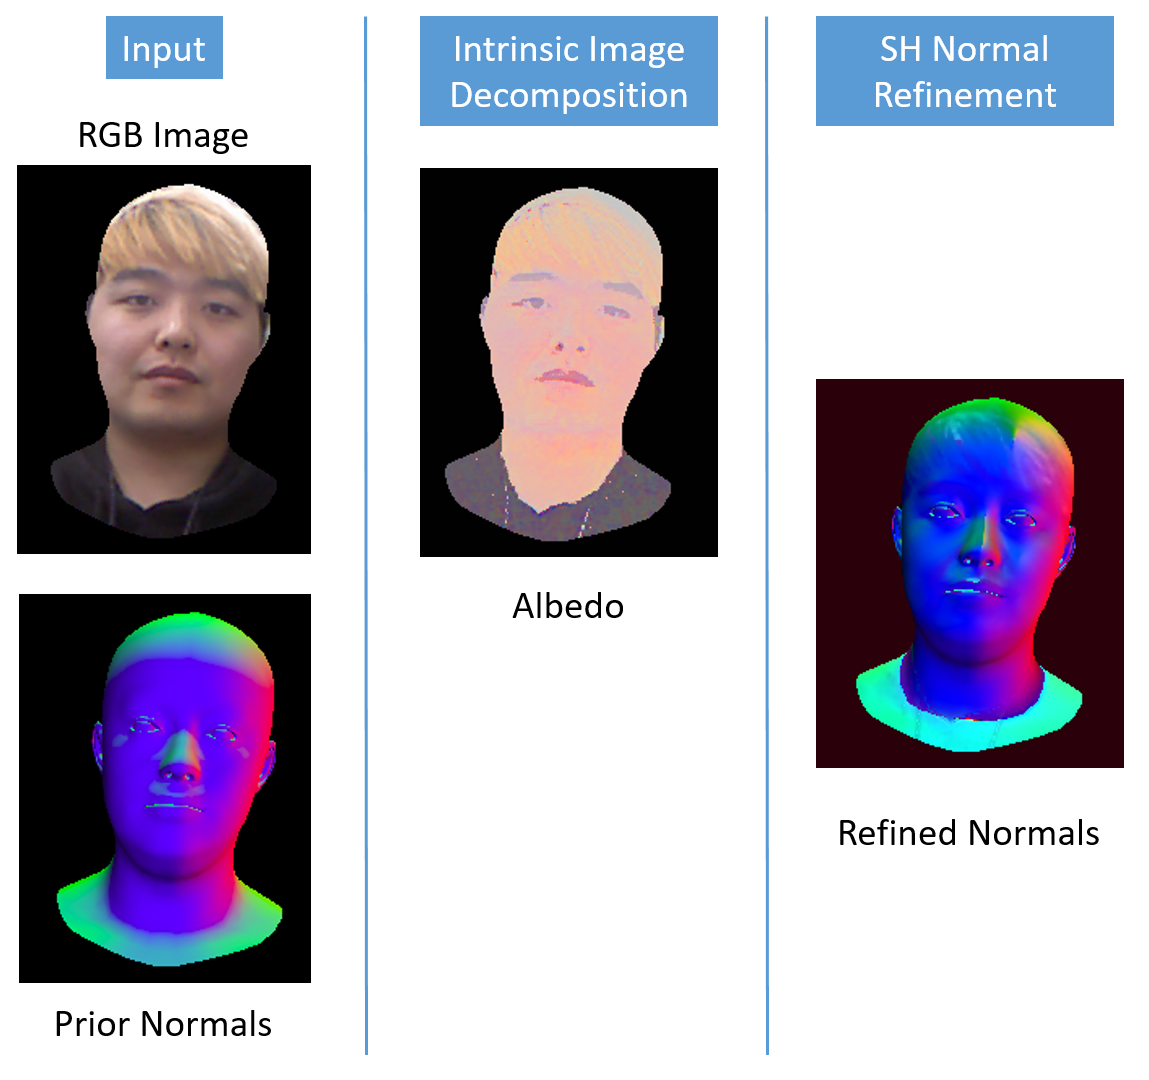
\includegraphics [scale=0.25] {image/refine_pipeline.png}
    \end{center}
    \caption{Refinement Pipeline: Inputs are raw RGB image $I$ and normals extracted from target geometry $N_{ref}$. First, intrinsic image decomposition of raw RGB image to get albedo $\rho$. Then solve for lighting using prior normal map $N_{ref}$ and albedo $\rho$. Finally, refine Normals $N$ using albedo $\rho$ and solved lighting parameters $L_l^m$.}
    \label{fig:pipe2}
\end{figure} 
We first solve for the unknown illumination parameters $L_l^m$ by minimizing the energy
\begin{equation}
\min_{L} I(u,v) - \rho(u,v) \sum_{l,m} a_l L_{lm} Y_{lm}(n_{ref}(u,v)).
\end{equation}
With illumination known, we next refine the prior normal map by minimizing
\begin{equation}
\min_{n} I(u,v) - \rho(u,v) \sum_{l,m} a_l L_{lm} Y_{lm}(n(u,v)).
\end{equation}

\section{Visualization}
To visualize our refined normal, we simply used a fragment shader with OpenGL. In the fragment shader, the illumination consists of 2nd-order spherical harmonics with greyscale values and one directional light. There are two ways of visualizing, the one is using our refined normal and the other one is just using simple interploated normal.  When we mapped the texture from the original image, the results didn't have big differences as Figure 6 shows. It is because the texture from the original image is already shaded. However, when we mapped the flat texture with gray color, the results had big differences as Figure 7 shows.  The result with our refined normal has much more details and looks much more realistic.


\begin{figure}[!h]
	\begin{center}
		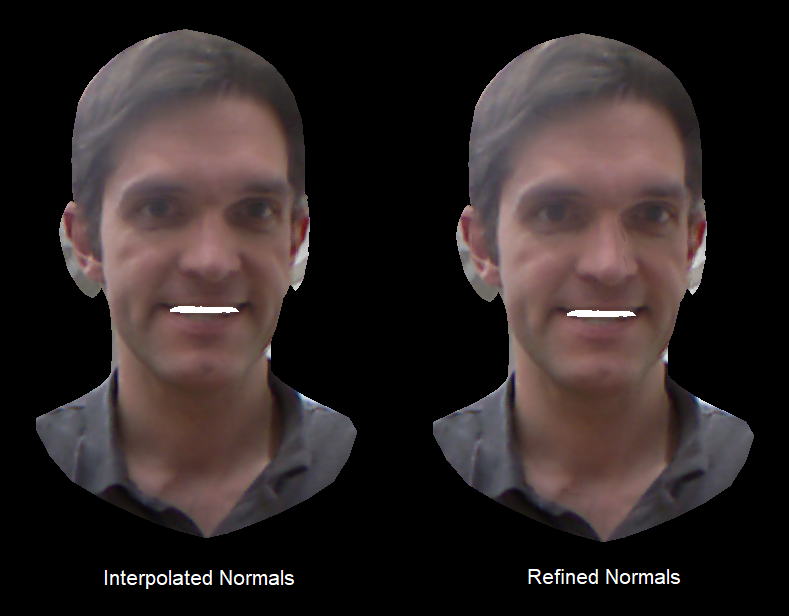
\includegraphics [scale=0.33] {image/visual1.png}
	\end{center}
	\caption{Visualized results with texture from the original image}
	\label{fig:result-visual1}
\end{figure} 

\begin{figure}[!h]
	\begin{center}
		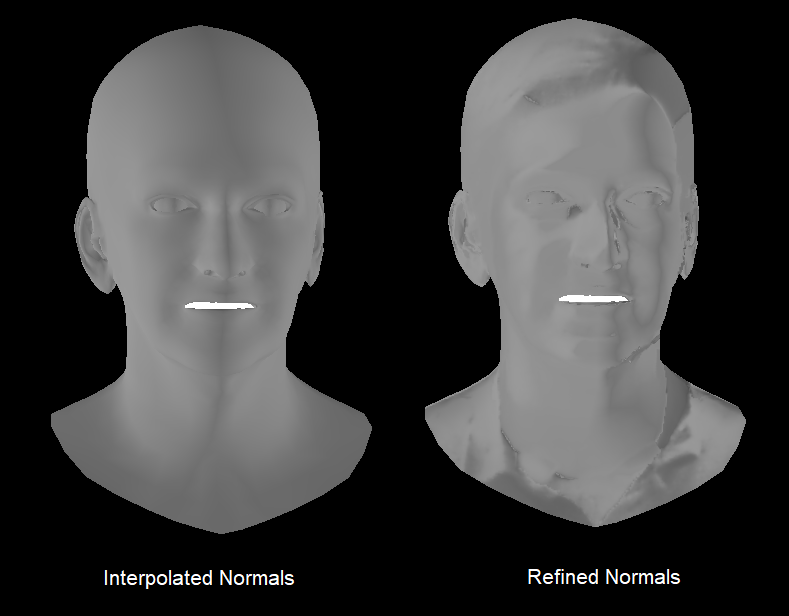
\includegraphics [scale=0.33] {image/visual2.png}
	\end{center}
	\caption{Visualized results with flat texture with gray color}
	\label{fig:result-visual2}
\end{figure} 

\section{Results}
\subsection{Normal Refinement}
The minimized illumination and per-pixel surface normals results in very small Least-Squared Error (LSE). This results in low error reproduction of the shading $s$ removed from the albedo $\rho$ during intrinsic image decomposition, see Fig. \ref{fig:grey}. 


\begin{figure}[!h]
    \begin{center}
        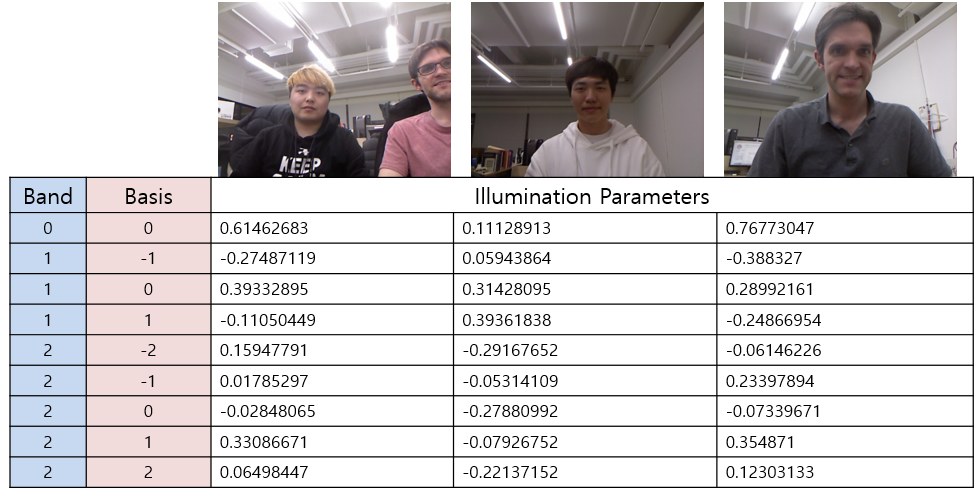
\includegraphics [scale=0.33] {image/illum.png}
    \end{center}
    \caption{Examples of solved SH illumination parameters $L_l^m$}
    \label{fig:result-illum}
\end{figure} 

\begin{figure}[!h]
\begin{center}
    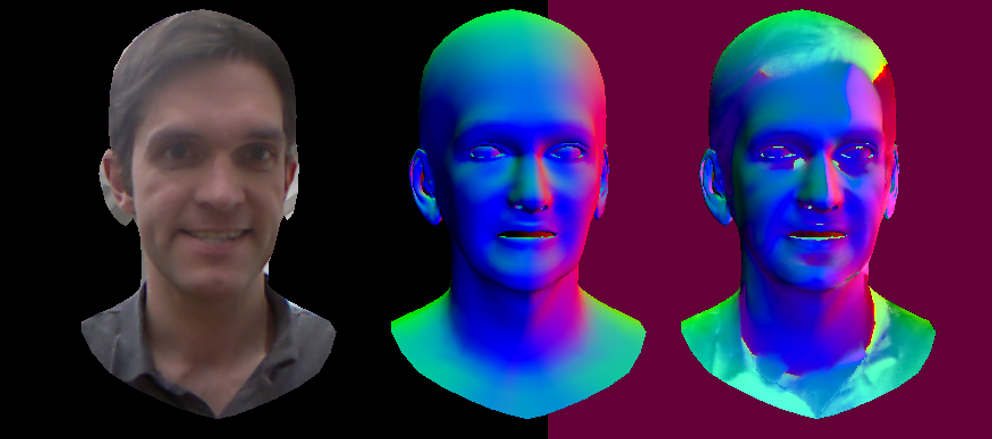
\includegraphics [scale=0.31] {image/normals1.png}
    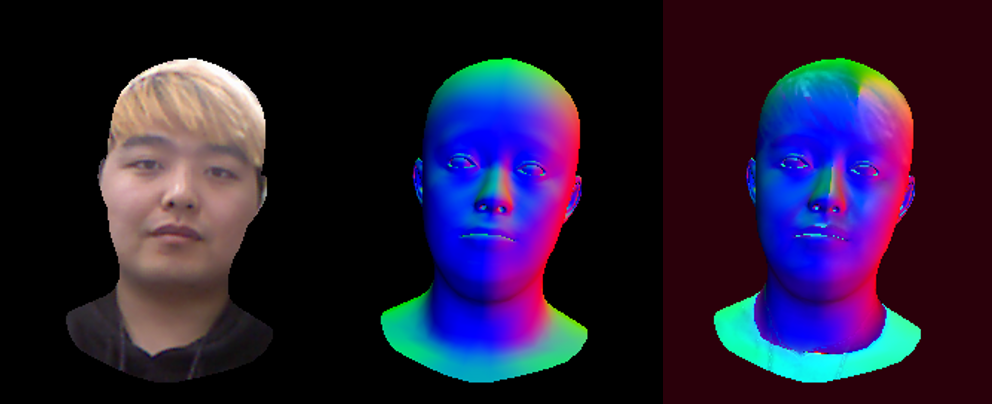
\includegraphics [scale=0.312] {image/normals2.png}
    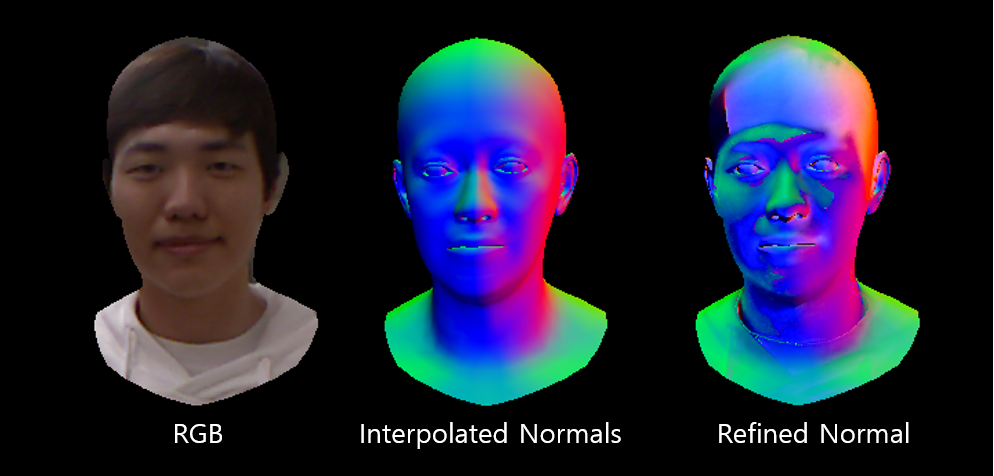
\includegraphics [scale=0.31] {image/normals3.png}
\end{center}
\caption{Results of refined normal maps}
\label{fig:normals}
\end{figure} 

\begin{figure}[!h]
    \begin{center}
        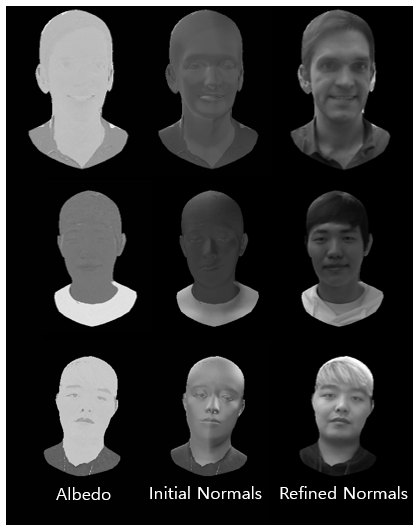
\includegraphics [scale=0.75] {image/grey-sh.png}
    \end{center}
    \caption{Shading realistically added using the same SH illumination parameters $L_l^m$. The results of illuminating the albedo with initial normals $N_{ref}$ and refined normals $N$. \textbf{Top:} LSE: 9.33e-10 \textbf{Middle:} LSE: 6.03e-09 \textbf{Bottom:} LSE: 3.75e-12}
    \label{fig:grey}
\end{figure} 
The resulting normal maps appear to better match the perceived geometry of the input image over the interpolated face model, see Fig. \ref{fig:normals}.

\subsection{Rendered Results} \label{sec:render}
The improved reflectance is clearly visible in the illuminated untextured (uniform color) face models. The rendered untextured models using interpolated normals clearly lack fine surface details. Rendered untextured models using the refined normal map have far more reflected detail added, including nose shape, improved eye shape, more details in all areas of the face and neck, with the addition fo hair and clothing not represented by the model. \par 
When texturing the face model using the RGB Image $I$, it is difficult to notice any improvements to due to the naturally illuminated image image. 
There is also some noise, this is caused by some loss in converting 32-bit floating point normals to unsigned char. We hope to fix this conversion issue, and we are currently seeing improvements in this area. Also regularization can help prevent some noise, to smooth sudden changes in surface normals. See Fig. \ref{fig:render} for result of renderings.


\begin{figure*}[t]
    \begin{center}
        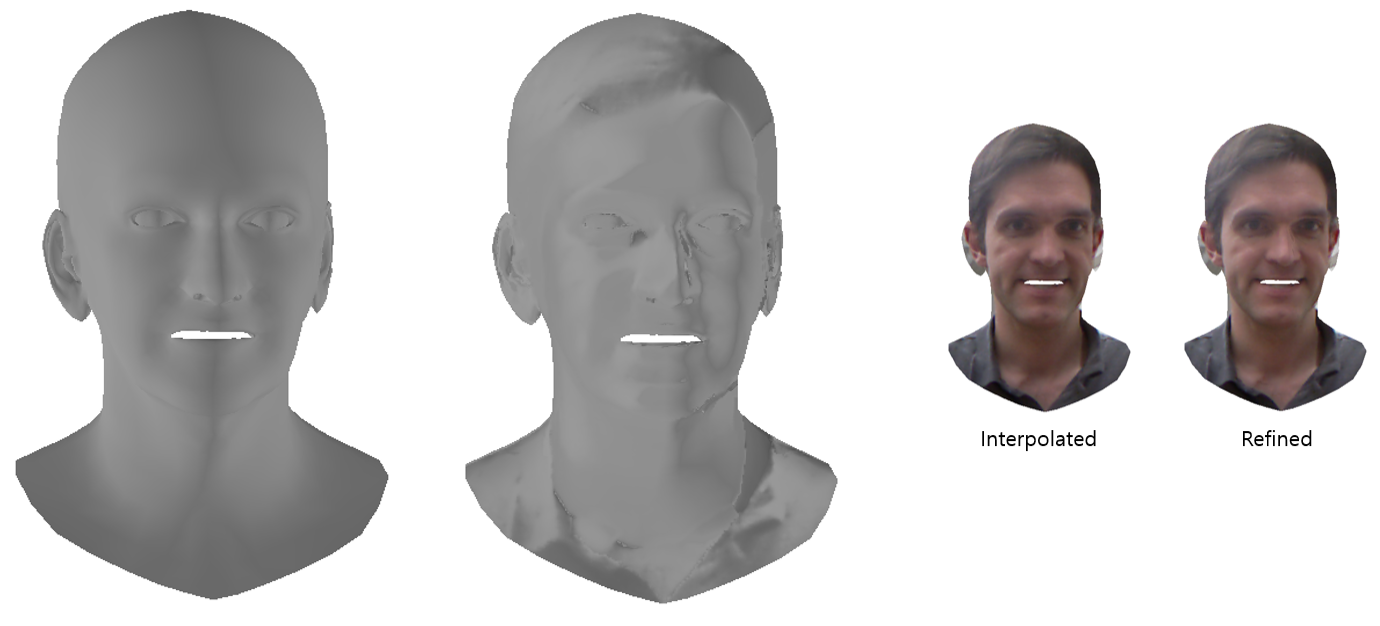
\includegraphics [scale=0.45] {image/render1.png}
        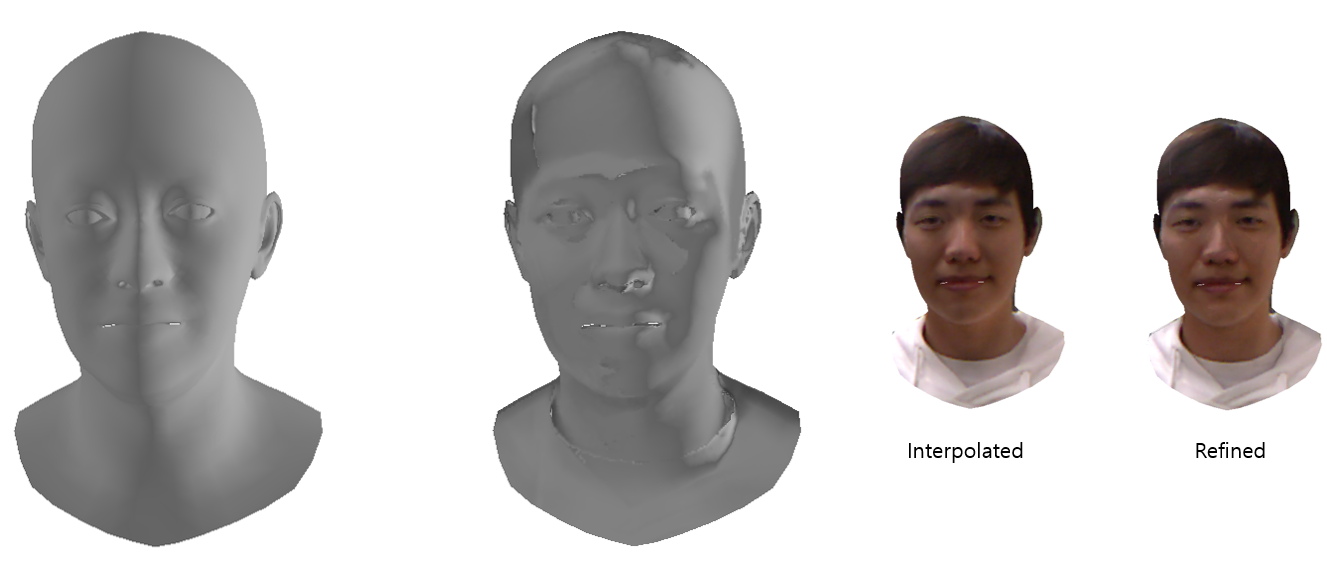
\includegraphics [scale=0.45] {image/render2.png}
        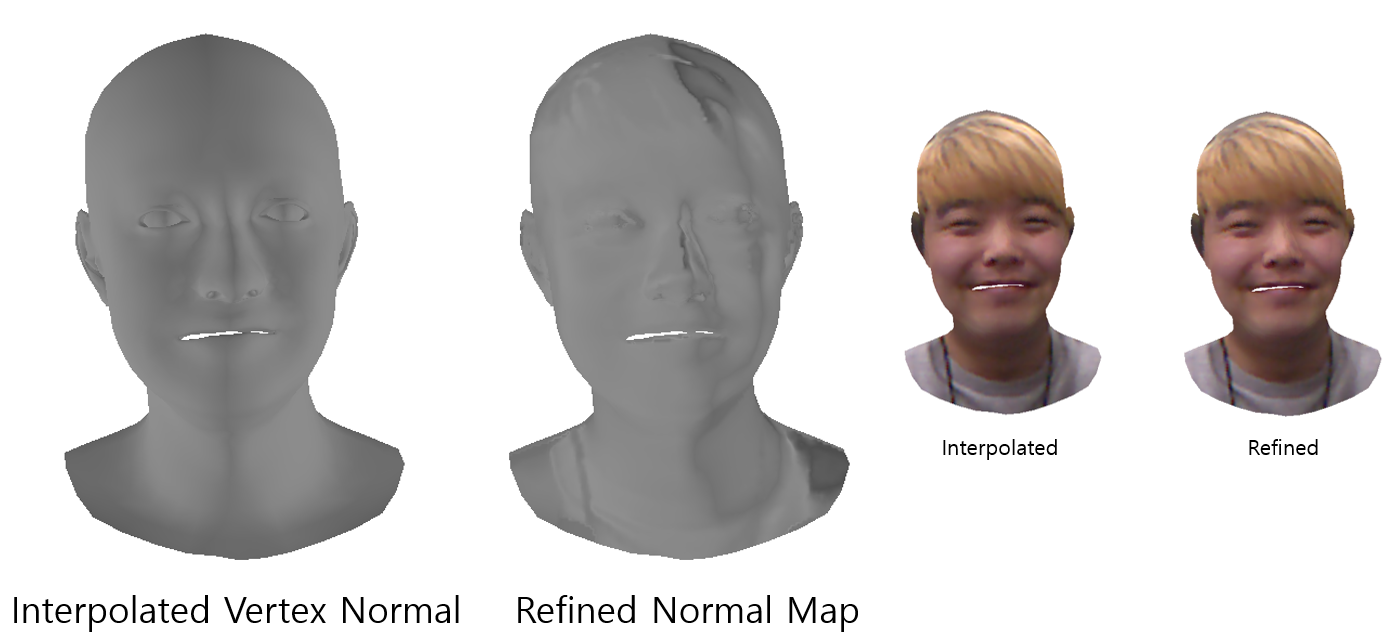
\includegraphics [scale=0.45] {image/render3.png}
    \end{center}
    \caption{OpenGL renderings under light source illuminates added normal details}
    \label{fig:render}
\end{figure*} 

\section{Team Member Roles}
See Table \ref{tab:roles}.
\begin{table}[!h]
	\begin{tabular}{l|l}
		\textbf{Name} & Roles \\
		\hline
		WonJong & Intrinsic Image Decomposition \\
		Dahun & Rendering: Model, Texture, and Normal Map \\
		Jake & Spherical Harmonics Normal Map Refinement \\
		\hline
	\end{tabular}
	\caption{Team Member Roles}
	\label{tab:roles}
\end{table}

\begin{thebibliography}{1}
	\bibitem{green} 
	R. Green.
	\textit{Spherical Harmonic Lighting: The Gritty Details}. 
	GDC 2003.
	
	\bibitem{dicky} 
	Rich Forster.
	\textit{Spherical Harmonics for Beginners}. 
	\url{https://dickyjim.wordpress.com/2013/09/04/spherical-harmonics-for-beginners/}

	\bibitem{igor} 
	Igor Goldvekht. 
	\textit{Shape-From-Shading}. 
	https://github.com/IgorGee/Shapes-From-Shading
    
    \bibitem{bell} 
    Sean Bell, Kavita Bala, Noah Snavely
    \textit{Intrinsic Images in the Wild}
     ACM Transactions on Graphics (SIGGRAPH 2014)
     \url{https://github.com/seanbell/intrinsic}
    
    \bibitem{sfs} 
    Ira Kemelmacher-Shlizerman, Member, IEEE, and Ronen Basri, Senior Member, IEEE \textit{3D Face Reconstruction from a Single Image Using a Single Reference Face Shape}
    IEEE TRANSACTIONS ON PATTERN ANALYSIS AND MACHINE INTELLIGENCE, VOL. 33, NO. 2, FEBRUARY 2011.
    
    \bibitem{pca} 
    Volker Blanz, Thomas Vetter
    \textit{A Morphable Model For The Synthesis Of 3D Faces}
    SIGGRAPH 1999
    
\end{thebibliography}

\end{document}
